% Provenance (never printed): see sources/outline_sources.md (Year 2: effusive and explosive
% eruptions, eruptive styles, eruption columns, pyroclastic deposits, explosivity index,
% volcano monitoring).
% Curves from figdata/bachelor-2/eruptions.py (closed-system gas fraction, Cotopaxi Layer 5
% thinning, GVP frequency-size law, column height fits, Mogi uplift); exercise and problem
% values in the Book 4 scratch calculators calc/ch06.py and calc/ch06pb.py.
\chapter{Erupsi Gunung Api}\label{ch:b2:eruptive-styles}

Pada 15 Juni 1991, Gunung Pinatubo di Filipina melontarkan lebih dari lima
kilometer kubik material; awan abunya naik hingga
\qty{35}{km}, puncaknya runtuh menjadi \omterm{def:b2:eruptive-styles:caldera}{kaldera} selebar \qty{2.5}{km}, dan
dua puluh juta ton belerang dioksida yang dimasukkannya ke stratosfer mendinginkan
seluruh dunia sekitar setengah derajat selama dua tahun. Seminggu sebelumnya, \omterm{def:b2:magma-emplacement:magma}{magma} pertama
yang mencapai permukaan sama sekali tidak berbuat demikian: setelah kehilangan sebagian besar
gasnya dalam perjalanan naik, \omterm{def:b2:magma-emplacement:magma}{magma} itu meleleh keluar sebagai \omterm{def:b2:eruptive-styles:dome}{kubah lava}. Di Kīlauea, Hawaii,
erupsi Pu`u~`\=O`\=o mencurahkan \qty{4.4}{km^3} lava, volume yang sebanding,
selama tiga puluh lima tahun, sebagai air mancur dan aliran yang menghancurkan 215 bangunan
tanpa pernah menaikkan kolom abu yang menjulang. Bumi yang sama, fisika yang sama, tiga perilaku: yang
membedakannya adalah seberapa banyak gas yang dibawa \omterm{def:b2:magma-emplacement:magma}{magma}, apakah gas itu dapat meninggalkan
lelehan dengan tenang, dan seberapa cepat \omterm{def:b2:magma-emplacement:magma}{magma} naik. Bab ini mengikuti sebuah erupsi
dari gelembung di dalam konduit hingga kolom di atas lubang kepundan dan endapan yang
ditinggalkannya, lalu mengukur erupsi, menghitungnya, dan mengamati gunung api untuk mencari
tanda-tanda bahwa sebuah erupsi akan datang.
% ledger: usgs:pinatubo-1991, usgs:puuoo

\begin{recall}
\textbf{Dari volume-volume sekolah}: gunung api, lubang kepundan dan kawahnya, dapur
\omterm{def:b2:magma-emplacement:magma}{magma} di bawahnya, lava, dan abu vulkanik. \textbf{Dari
\cref{ch:b2:magma-emplacement}}: \omterm{def:b2:magma-emplacement:volatiles}{volatil magmatik}, eksolusinya di bawah
tekanan jenuh, hukum akar kuadrat kelarutan air $w = s\sqrt p$ dengan
$s \approx 0.34$ persen per $\sqrt{\unit{MPa}}$ untuk basal dan $0.44$ untuk
riolit, serta viskositas lelehan, yang terpaut sepuluh orde besaran.
\textbf{Dari buku-buku fisika}: hukum gas ideal $pV = nRT$; daya apung;
analisis dimensi, yang membangun satu-satunya kombinasi besaran yang diberikan
yang berdimensi sama dengan jawabannya; jangkauan proyektil, $v^2\sin 2\theta/g$
tanpa hambatan udara. \textbf{Dari buku-buku matematika}: proses Poisson,
tempat peristiwa-peristiwa independen dengan laju tetap $\lambda$ memberikan sedikitnya satu peristiwa
dalam waktu $t$ dengan peluang $1 - e^{-\lambda t}$; garis lurus kuadrat terkecil.
Dari volume Tahun 1: gempa bumi dan magnitudonya.
\end{recall}

\section{Efusif atau eksplosif}

\begin{definition}[Erupsi efusif dan eksplosif, fragmentasi]\label{def:b2:eruptive-styles:regimes}
Yang disebut \emph{erupsi efusif}\index{erupsi efusif} adalah erupsi yang didominasi oleh
pencurahan lava, yang mengalir menjauhi lubang kepundan sebagai cairan yang utuh. Yang disebut
\emph{erupsi eksplosif}\index{erupsi eksplosif} terutama menghasilkan fragmen,
abu, batu apung, dan puing balistik, yang dibawa oleh gas yang mengembang. Yang disebut \emph{fragmentasi
magma}\index{fragmentasi magma} adalah pecahnya lelehan kontinu
yang mengandung gelembung menjadi gas kontinu yang membawa tetesan dan fragmen lelehan;
fragmentasi mengubah aliran efusif menjadi aliran eksplosif.
\end{definition}
% ledger: usgs:glossary-ch6, cassidy18:fragmentation

Yang menggerakkan peralihan itu adalah gas. \omterm{def:b2:magma-emplacement:magma}{Magma} yang naik dari kedalaman membawa
air dan karbon dioksida terlarut; di bawah tekanan jenuhnya, volatil-volatil itu
keluar dari larutan sebagai gelembung, dan gelembung mengembang ketika tekanan turun.
Jika gelembung tetap berada dalam lelehan, gas segera mengisi sebagian besar volume.

\begin{proposition}[Fraksi volume gas pada pelepasan gas sistem tertutup]\label{prop:b2:eruptive-styles:gas}
Misalkan sebuah \omterm{def:b2:magma-emplacement:magma}{magma} mengandung fraksi massa air $w_0$, dengan kelarutan $w(p) =
s\sqrt p$, dan misalkan air yang tereksolusi tetap bersama lelehan sebagai gas
ideal pada suhu $T$. Di bawah tekanan jenuh $p_s = (w_0/s)^2$, satu
kilogram \omterm{def:b2:magma-emplacement:magma}{magma} memuat $x = w_0 - s\sqrt p$ kilogram uap, dan fraksi
volume gasnya adalah
\[
\phi(p) = \frac{V_g}{V_g + V_m}, \qquad V_g = \frac{x\,RT}{M p}, \qquad
V_m = \frac{1 - x}{\rho_m},
\]
dengan $M = \qty{0.018}{kg/mol}$ massa molar air dan $\rho_m$ massa jenis
lelehan.
\end{proposition}

\begin{proof}
Di atas $p_s$ lelehan dapat menampung seluruh airnya dan tidak ada gas. Di bawah $p_s$
lelehan hanya mempertahankan kelarutannya $s\sqrt p$, sehingga massa $x = w_0 - s\sqrt p$ per
kilogram \omterm{def:b2:magma-emplacement:magma}{magma} berupa uap. Uap itu, $x/M$ mol, menempati $xRT/(Mp)$ menurut
hukum gas ideal; sisa $1 - x$ kilogram lelehan menempati $(1 - x)/\rho_m$.
Fraksi volumenya menyusul.
\end{proof}
% ledger: moore98:h2o

Karena $V_g$ bertambah sebagai $1/p$, buih itu mengembang paling cepat di dekat permukaan.
Gambar di bawah mengikuti riolit dengan \qty{5}{\percent} air dan basal
dengan \qty{1}{\percent}. Riolit itu jenuh pada \qty{127}{MPa}, sekitar
\qty{5}{km} di bawah; pada \qty{10}{MPa} gasnya sudah mengisi \qty{82}{\percent}
volume. Dalam sebuah model aliran konduit yang telah diterbitkan, \omterm{def:b2:magma-emplacement:magma}{magma} terfragmentasi ketika
gas mengisi \qty{85}{\percent} volumenya, tingkat yang dicapai riolit ini pada
\qty{8.2}{MPa}, sekitar \qty{330}{m} di bawah lubang kepundan untuk gradien tekanan
\qty{0.025}{MPa/m}. Basal itu baru jenuh pada \qty{8.7}{MPa} dan mencapai
buih yang sama pada \qty{1.8}{MPa}, dalam jarak seratus meter dari permukaan.
% ledger: cassidy18:fragmentation, cassidy18:ascent

\begin{omfigure}
\centering
\begin{tikzpicture}
\begin{axis}[omrecord, width=0.82\linewidth, height=5.6cm, xmode=log,
  xmin=0.01, xmax=200, ymin=0, ymax=1,
  xlabel={tekanan (\unit{MPa})}, ylabel={fraksi volume gas $\phi$},
  legend pos=south west, legend style={font=\scriptsize},
  tick label style={font=\scriptsize}, label style={font=\small}]
\addplot[very thick, red!70!black] table[x=p_MPa, y=rhyolite] {figdata/out/bachelor-2-eruptions-gas.dat};
\addlegendentry{riolit, \qty{5}{\percent} H$_2$O, \qty{850}{\celsius}}
\addplot[very thick, black, dashed] table[x=p_MPa, y=basalt] {figdata/out/bachelor-2-eruptions-gas.dat};
\addlegendentry{basal, \qty{1}{\percent} H$_2$O, \qty{1200}{\celsius}}
\draw[densely dotted, thick, gray] (axis cs:0.01,0.85) -- (axis cs:200,0.85);
\node[anchor=north west, font=\scriptsize, inner sep=1pt] at (axis cs:0.012,0.835) {fragmentasi dalam model konduit};
\end{axis}
\end{tikzpicture}
\par\smallskip{\small Fraksi volume uap air yang tereksolusi terhadap tekanan
pada pelepasan gas sistem tertutup (\cref{prop:b2:eruptive-styles:gas}), dengan hukum
kelarutan dari \cref{ch:b2:magma-emplacement}. Tekanan turun ke kiri, seiring \omterm{def:b2:magma-emplacement:magma}{magma}
naik; garis bertitik menandai fraksi gas tempat sebuah model konduit yang telah diterbitkan
memfragmentasi \omterm{def:b2:magma-emplacement:magma}{magma}.}
\end{omfigure}
% ledger: moore98:h2o, cassidy18:fragmentation

Jadi basal pun akan terfragmentasi jika gasnya tetap berada di dalamnya; dan dalam air mancur lava
Hawaii hal itu memang terjadi, di dekat lubang kepundan. Yang membuat sebagian besar erupsi basal lemah adalah bahwa
gas tidak harus tinggal. Dalam lelehan berviskositas rendah, gelembung naik melalui
cairan, bergabung, dan lolos, dan begitu gelembung-gelembung tersambung menjadi jaringan yang permeabel,
yang terjadi pada fraksi gas antara \qty{30}{\percent} dan \qty{78}{\percent}
dalam eksperimen, gas merembes keluar melalui dinding dan lubang kepundan tanpa membawa
lelehan: \omterm{def:b2:magma-emplacement:magma}{magma} melepaskan gas dalam sistem terbuka dan mencapai permukaan sebagai
lava. \omterm{def:b2:magma-emplacement:magma}{Magma} yang kental justru menahan gelembungnya dan terfragmentasi, lelehannya pecah
seperti kaca ketika diregangkan lebih cepat daripada kemampuannya mengalir. Laju kenaikan menentukan
pilihan di antara keduanya sama besarnya dengan komposisi: pada banyak erupsi, aktivitas efusif
berpasangan dengan laju dekompresi sekitar \qty{0.0001}{MPa/s} dan \omterm{def:b2:eruptive-styles:regimes}{erupsi eksplosif}
dengan laju sekitar \qty{1}{MPa/s}, dan perubahan viskositas lelehan sebesar setengah
satuan logaritmik, kira-kira faktor tiga, dapat menggeser erupsi dari satu rezim ke
rezim lainnya. \omterm{def:b2:eruptive-styles:dome}{Kubah lava} pertama Pinatubo dan erupsi puncaknya seminggu kemudian
berasal dari \omterm{def:b2:magma-emplacement:magma}{magma} yang sama: kelompok pertama sempat kehilangan gasnya, kelompok berikutnya tidak.
% ledger: cassidy18:fragmentation, cassidy18:ascent, usgs:pinatubo-1991

Air dari luar melakukan apa yang dilakukan gas \omterm{def:b2:magma-emplacement:magma}{magma} itu sendiri. Air tanah, danau, atau
laut yang bertemu \omterm{def:b2:magma-emplacement:magma}{magma} seketika berubah menjadi uap, dan pengembangan air yang
sangat panas itu menghancurkan \omterm{def:b2:magma-emplacement:magma}{magma}: eksperimen menunjukkan bahwa lebih dari \qty{30}{\percent}
panas yang tersedia dapat diubah menjadi energi mekanik. \omterm{def:b2:magma-emplacement:magma}{Magma} yang miskin gas pun
kemudian dapat meletus secara eksplosif.
% ledger: cassidy18:fragmentation

\section{Gaya erupsi}

Ahli vulkanologi menamai erupsi menurut contoh-contoh klasik. Nama-nama itu menggambarkan rupa
sebuah erupsi, dan saling bergradasi; satu erupsi sering melewati
beberapa gaya.

\begin{definition}[Gaya erupsi]\label{def:b2:eruptive-styles:styles}
Menurut eksplosivitas yang makin besar, di antara erupsi yang digerakkan oleh gas \omterm{def:b2:magma-emplacement:magma}{magma} itu sendiri:
\begin{itemize}
\item \emph{erupsi Hawaii}\index{erupsi Hawaii} menghasilkan air mancur
lava basal yang sangat encer, setinggi puluhan hingga ratusan meter, yang memasok aliran lava;
\item \emph{erupsi Stromboli}\index{erupsi Stromboli} adalah serangkaian
letupan terpisah yang melontarkan gumpalan pijar \omterm{def:b2:magma-emplacement:magma}{magma} basal hingga
andesit basaltik sampai setinggi sekitar seratus meter, tanpa kolom
yang berkelanjutan;
\item \emph{erupsi Vulkano}\index{erupsi Vulkano} adalah ledakan singkat dan dahsyat
gas yang terkumpul di bawah sumbat lava yang telah membeku, yang menghancurkan
sumbat itu dan melontarkan blok serta kolom gelap abu halus, umumnya dari
\omterm{def:b2:magma-emplacement:magma}{magma} menengah;
\item \emph{erupsi Plini}\index{erupsi Plini} adalah semburan berkelanjutan gas
dan \omterm{def:b2:magma-emplacement:magma}{magma} yang terfragmentasi, biasanya silikat, yang memasok kolom yang naik ke
stratosfer selama berjam-jam hingga berhari-hari dan menyebarkan lapisan batu apung dan abu di atas
ribuan kilometer persegi.
\end{itemize}
Jika air dari luar yang menggerakkan fragmentasi, \emph{erupsi
freatomagmatik}\index{erupsi freatomagmatik} melontarkan uap bersama fragmen
\omterm{def:b2:magma-emplacement:magma}{magma} segar, sedangkan \emph{erupsi freatik}\index{erupsi freatik} adalah
ledakan yang digerakkan uap dari air tanah atau air permukaan yang dipanaskan oleh \omterm{def:b2:magma-emplacement:magma}{magma} atau batuan panas,
yang melontarkan uap dan fragmen batuan yang lebih tua tetapi tanpa \omterm{def:b2:magma-emplacement:magma}{magma} segar.
\end{definition}
% ledger: nps:styles, usgs:glossary-ch6

Setiap gaya memiliki erupsi tipenya. Pu`u~`\=O`\=o, di Kīlauea, bergaya Hawaii selama sebagian besar
tiga puluh lima tahun dan enam puluh satu episodenya, dengan air mancur yang umumnya naik
\qtyrange{10}{100}{m} dan sesekali lebih dari \qty{500}{m}. Stromboli,
``mercusuar Laut Tengah'', memberikan namanya pada letupan-letupan yang membangun
kerucut sinder. Ledakan Vulkano mengguncang Trident di Alaska secara berselang antara
1953 dan 1974. Vesuvius pada tahun 79 M, yang digambarkan oleh Plinius Muda, memberikan namanya pada
\omterm{def:b2:eruptive-styles:styles}{erupsi Plini}; Gunung St.~Helens pada 18~Mei~1980 dan Novarupta pada tahun 1912, yang
kolomnya naik di atas \qty{30}{km} dalam erupsi yang berlangsung hampir tiga hari, adalah
contoh-contoh modern.
Kasus-kasus antara dengan kolom di bawah sekitar \qty{20}{km}, berkelanjutan tetapi tidak tunak,
disebut sub-Plini. Dengan air, \omterm{def:b2:eruptive-styles:styles}{erupsi Stromboli} menjadi erupsi Surtsey,
yang dinamai menurut erupsi Surtsey tahun 1963 di lepas pantai Islandia, dan membangun cincin
tuf yang rendah dan maar; \omterm{def:b2:eruptive-styles:styles}{erupsi Plini} menjadi freatoplini. Di Pinatubo, ledakan
uap menghasilkan tiga kawah di lereng utara pada bulan Maret dan April 1991, dua
bulan sebelum erupsi puncak: ledakan-ledakan itu freatik.
% ledger: nps:styles, usgs:puuoo, usgs:glossary-ch6, usgs:pinatubo-deposits

\begin{definition}[Kubah lava]\label{def:b2:eruptive-styles:dome}
Yang disebut \emph{kubah lava}\index{kubah lava} adalah gundukan berlereng terjal dari lava kental,
umumnya dasit atau riolit, yang terekstrusi perlahan dari lubang kepundan dan menumpuk di atasnya
alih-alih mengalir menjauh.
\end{definition}
% ledger: usgs:glossary-ch6

Kubah adalah apa yang dibuat \omterm{def:b2:magma-emplacement:magma}{magma} kental ketika telah kehilangan gasnya: \omterm{def:b2:magma-emplacement:magma}{magma} pertama Pinatubo
pada Juni 1991, dan kubah yang tumbuh di kawah Gunung St.~Helens dalam
tujuh belas episode antara 1980 dan 1986 hingga \qty{267}{m} di atas dasar kawah.
Kubah juga dapat menjadi sumbat yang di bawahnya ledakan Vulkano berikutnya terbangun,
dan keruntuhannya dapat melepaskan tekanan pada \omterm{def:b2:magma-emplacement:magma}{magma} kaya gas di bawahnya. Foto-foto
di bawah menunjukkan kedua ujung rentang itu.
% ledger: usgs:pinatubo-1991, usgs:msh-dome, cassidy18:fragmentation

\begin{omfigure}
\centering
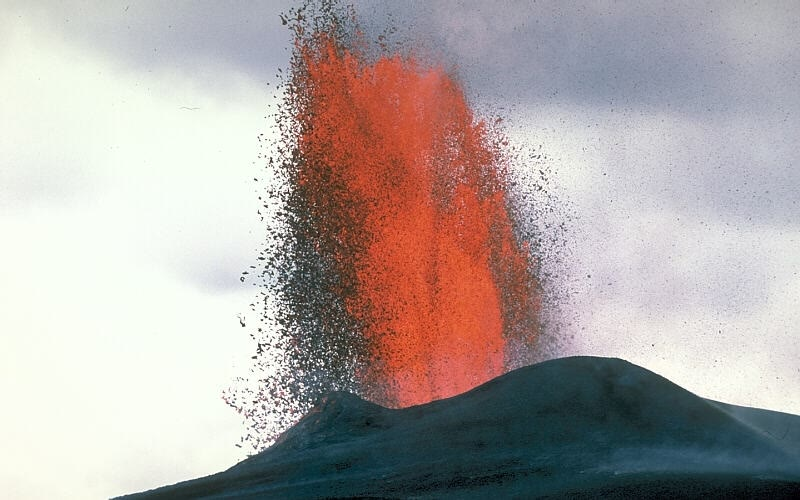
\includegraphics[height=4.3cm]{images/book4/b2-kilauea-fountain.jpg}\hfill
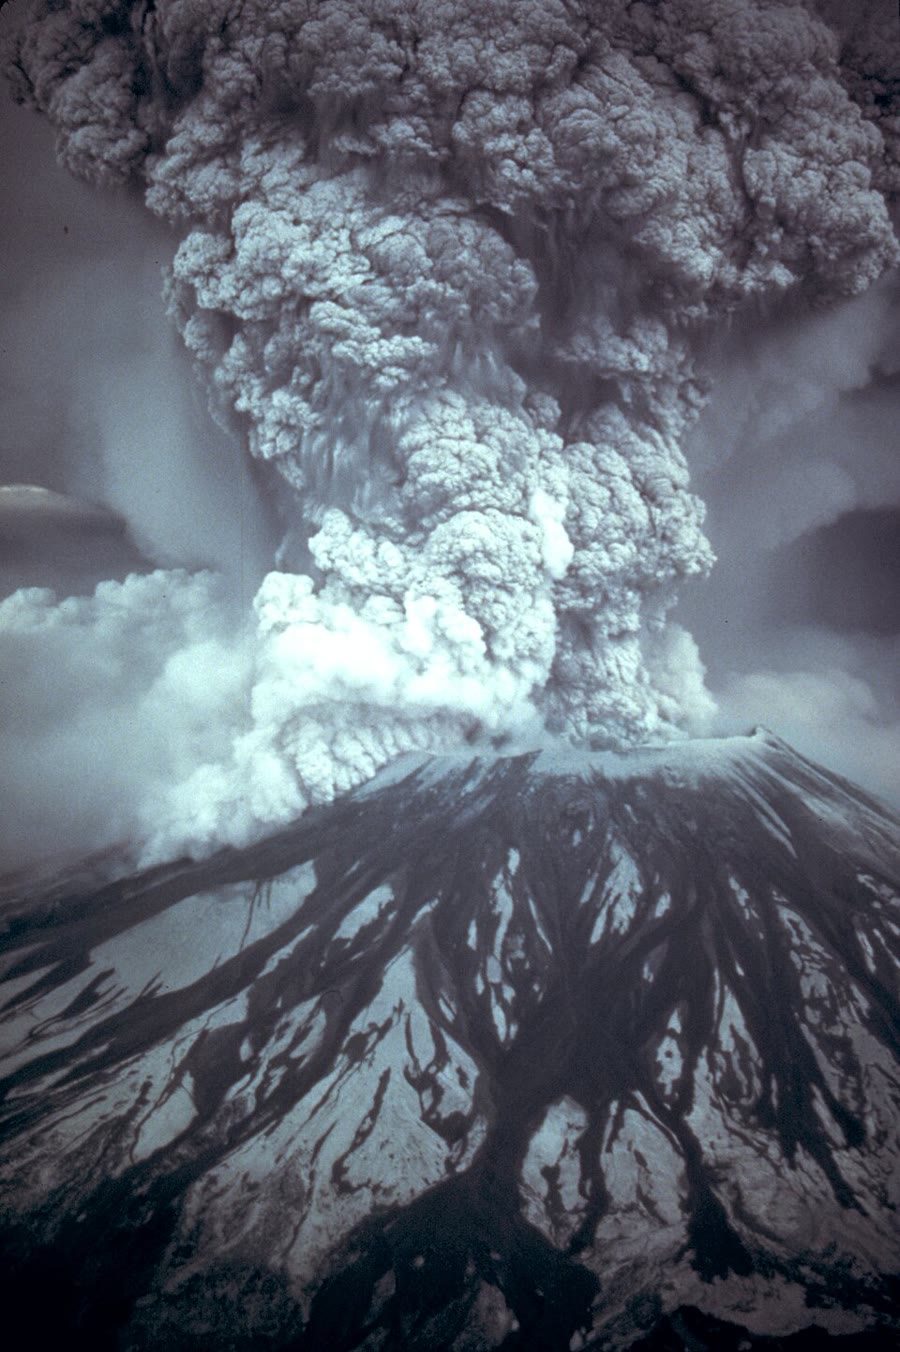
\includegraphics[height=4.3cm]{images/book4/b2-st-helens-column.jpg}\hfill
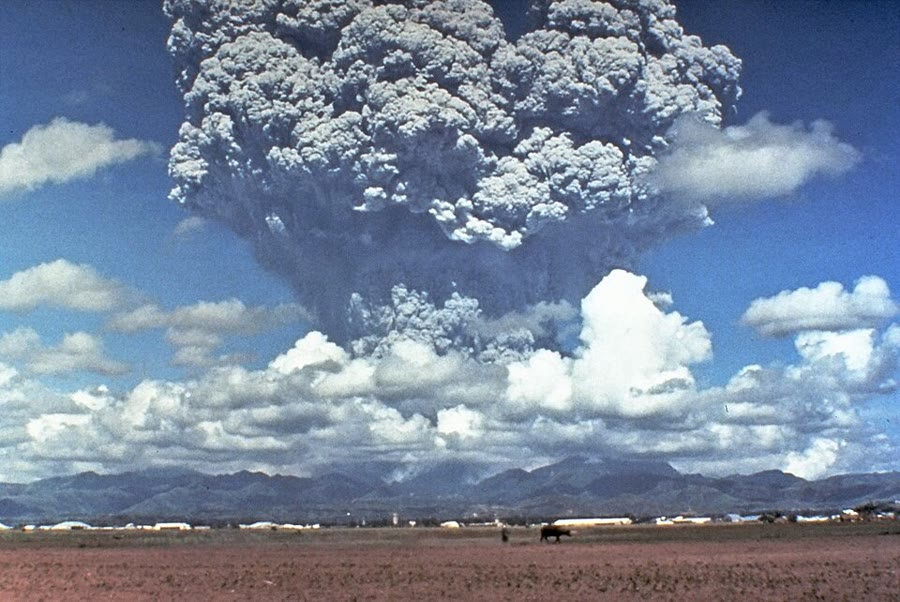
\includegraphics[height=4.3cm]{images/book4/b2-pinatubo-column.jpg}
\par\smallskip{\small Kiri: air mancur Hawaii di kerucut Pu`u~`\=O`\=o, Kīlauea,
Oktober 1983 (J.\,D.~Griggs, USGS). Tengah: kolom Plini Gunung St.~Helens,
18 Mei 1980 (Austin Post, USGS). Kanan: \omterm{def:b2:eruptive-styles:column}{kolom erupsi} Gunung Pinatubo pada
12 Juni 1991, tiga hari sebelum erupsi puncak (Dave Harlow, USGS). Ketiga
foto itu berada dalam domain publik.}
\end{omfigure}
% ledger: usgs:puuoo, usgs:msh-may18, usgs:pinatubo-1991

\section{Kolom erupsi}

\begin{definition}[Kolom erupsi]\label{def:b2:eruptive-styles:column}
Yang disebut \emph{kolom erupsi}\index{kolom erupsi} adalah massa gas dan
fragmen yang naik di atas lubang kepundan yang eksplosif. Kolom itu memiliki tiga bagian: \emph{semburan},
atau daerah dorongan gas, tempat campuran meninggalkan lubang kepundan dengan cepat tetapi lebih rapat daripada
udara dan naik oleh momentumnya; daerah \emph{konvektif}, tempat campuran,
setelah menelan dan memanaskan cukup banyak udara sehingga menjadi lebih ringan daripada sekelilingnya,
naik oleh daya apung; dan awan \emph{payung}, yang menyebar ke samping pada
ketinggian tempat massa jenis kolom sama dengan massa jenis atmosfer.
\end{definition}
% ledger: usgs:glossary-ch6, nps:styles, aubry23:fits

\begin{omfigure}
\centering
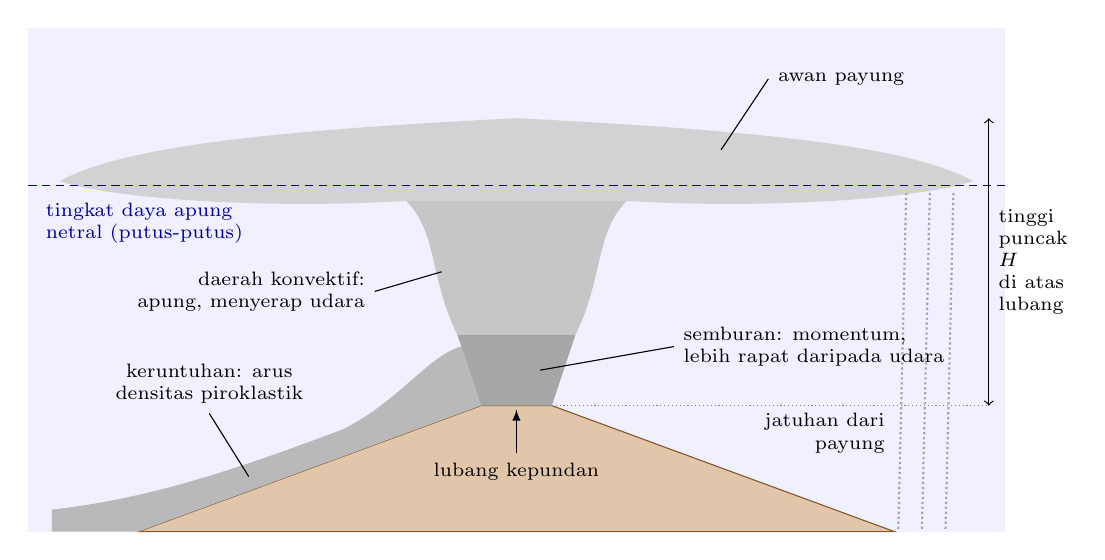
\begin{tikzpicture}[x=1cm, y=1cm, font=\scriptsize]
% atmosphere and ground
\fill[blue!6] (-6.2,0) rectangle (6.2,6.4);
% volcano
\fill[brown!45, draw=brown!70!black] (-4.8,0) -- (-0.45,1.6) -- (0.45,1.6) -- (4.8,0) -- cycle;
% collapse branch (left): a density current hugging the flank
\fill[gray!55] (-0.45,1.6) -- (-0.7,2.35) .. controls (-1.1,2.25) and (-1.5,1.65) .. (-2.2,1.3)
  .. controls (-3.4,0.85) and (-4.6,0.42) .. (-5.9,0.28) -- (-5.9,0) -- (-4.8,0) -- cycle;
% jet
\fill[gray!70] (-0.45,1.6) -- (0.45,1.6) -- (0.75,2.5) -- (-0.75,2.5) -- cycle;
% convective column
\fill[gray!45] (-0.75,2.5) .. controls (-1.1,3.2) and (-1.0,3.8) .. (-1.4,4.2)
  -- (1.4,4.2) .. controls (1.0,3.8) and (1.1,3.2) .. (0.75,2.5) -- cycle;
% umbrella
\fill[gray!35] (-1.4,4.2) .. controls (-3,4.1) and (-5,4.2) .. (-5.8,4.45)
  .. controls (-5,4.9) and (-3,5.1) .. (0,5.25) .. controls (3,5.1) and (5,4.9) .. (5.8,4.45)
  .. controls (5,4.2) and (3,4.1) .. (1.4,4.2) -- cycle;
\draw[densely dashed, blue!60!black] (-6.2,4.4) -- (6.2,4.4);
% fallout from the far end of the umbrella, down to the ground
\foreach \x in {4.95,5.25,5.55} {\draw[gray!70, densely dotted, thick] (\x,4.3) -- (\x-0.1,0.02);}
\draw[gray, densely dotted] (0.45,1.6) -- (6.0,1.6);
\draw[<->] (6.0,1.6) -- (6.0,5.25) node[midway, right, align=left] {tinggi\\puncak\\$H$\\di atas\\lubang};
% labels
\node[anchor=north west, align=left, blue!60!black] at (-6.1,4.3) {tingkat daya apung\\netral (putus-putus)};
\draw (-0.95,3.3) -- (-1.8,3.05) node[left, align=right] {daerah konvektif:\\apung, menyerap udara};
\draw (0.3,2.05) -- (2.0,2.35) node[right, align=left] {semburan: momentum,\\lebih rapat daripada udara};
\draw (2.6,4.85) -- (3.2,5.75) node[right] {awan payung};
\node[anchor=east, align=right] at (4.8,1.25) {jatuhan dari\\payung};
\draw (-3.4,0.7) -- (-3.9,1.5) node[above, align=center] {keruntuhan: arus\\densitas piroklastik};
\draw[-latex] (0,1.0) -- (0,1.55);
\node[anchor=north] at (0,1.0) {lubang kepundan};
\end{tikzpicture}
\par\smallskip{\small Anatomi \omterm{def:b2:eruptive-styles:column}{kolom erupsi} (skematis, tidak menurut skala). Di
kanan, kolom naik melewati ketiga daerahnya dan awan payung
menjatuhkan \omterm{def:b2:eruptive-styles:tephra}{tefra} sambil menyebar; di kiri, sebagian semburan gagal menjadi
apung dan runtuh menjadi \omterm{def:b2:eruptive-styles:pdc}{arus densitas piroklastik}.}
\end{omfigure}

Seberapa tinggi sebuah kolom naik terutama bergantung pada berapa banyak panas yang dibawanya setiap
sekon, yaitu pada laju erupsi massa~$Q$. Analisis dimensi memberikan
bentuk hukumnya.

\begin{proposition}[Tinggi plume apung]\label{prop:b2:eruptive-styles:plume}
Jika tinggi puncak $H$ sebuah plume apung di atas sumber titik yang tunak hanya bergantung
pada fluks daya apung sumber $F$ (berdimensi $\mathrm{m^4\,s^{-3}}$) dan pada
frekuensi daya apung $N$ atmosfer yang terstratifikasi stabil (berdimensi
$\mathrm{s^{-1}}$), maka
\[
H = c\,F^{1/4}N^{-3/4}
\]
dengan $c$ konstanta tak berdimensi. Karena $F$ sebanding dengan fluks panas, dan karena itu
dengan laju erupsi massa, $H \propto Q^{1/4}$ dalam atmosfer tertentu.
\end{proposition}

\begin{proof}
Tuliskan $H = c\,F^{\alpha}N^{\beta}$. Menyamakan panjang memberikan $4\alpha = 1$; menyamakan
waktu memberikan $-3\alpha - \beta = 0$. Karena itu $\alpha = 1/4$ dan $\beta = -3/4$, dan tidak ada
kombinasi lain $F$ dan $N$ yang berdimensi panjang.
\end{proof}

Konstanta $c$ berasal dari seberapa cepat plume menelan udara, yang dalam teori plume
diperlakukan dengan koefisien penyeretan yang diukur dalam eksperimen; konstanta itu diterima
di sini. Kolom nyata bukan sumber titik yang tunak dalam atmosfer yang tenang, sehingga
ahli vulkanologi mencocokkan hukum itu dengan erupsi yang tinggi dan laju erupsi massanya
sama-sama terukur.
% ledger: aubry23:fits

\begin{proposition}[Tinggi kolom dan laju erupsi massa]\label{prop:b2:eruptive-styles:mastin}
Untuk tinggi puncak $H$ di atas lubang kepundan dalam kilometer dan laju erupsi massa
$Q$ dalam kilogram per sekon, kompilasi erupsi yang terdokumentasi baik memberikan
\[
H = 0.304\,Q^{0.241},
\]
dan himpunan data independen yang lebih besar, berisi 130 peristiwa, memberikan $H = 0.345\,Q^{0.226}$.
Sebarannya besar: galat akar rata-rata kuadrat relatif pada $H$ adalah
\qtyrange{53}{60}{\percent}.
\end{proposition}
\admitted
% ledger: aubry23:fits

Kedua eksponen itu dekat dengan $1/4$ teori plume. Gambar di bawah menunjukkan
kedua kecocokan itu dan contoh-contoh erupsi yang menjadi dasar parameter sumber yang dipakai
pusat-pusat prakiraan abu. Kolom setinggi \qty{15}{km}, seperti kolom Gunung
St.~Helens, memerlukan \qty{e7}{kg/s}, sepuluh ribu ton setiap sekon; menggandakan
tingginya memerlukan laju hampir delapan belas kali lipat. Dibaca sebaliknya, tinggi yang terukur memberikan
lajunya, tetapi hanya dalam batas faktor beberapa kali, karena $Q$ sebanding dengan $H^4$
(\cref{exo:b2:eruptive-styles:3}). Ahli vulkanologi menyatakan laju itu dengan \emph{intensitas} $I =
\log_{10}Q + 3$, dengan $Q$ dalam kilogram per sekon.
% ledger: mastin09:examples, aubry23:fits, brown14:record

\begin{omfigure}
\centering
\begin{tikzpicture}
\begin{axis}[omrecord, width=0.82\linewidth, height=6cm, xmode=log, ymode=log,
  xmin=1e3, xmax=1e9, ymin=1, ymax=60,
  xlabel={laju erupsi massa $Q$ (\unit{kg/s})}, ylabel={tinggi puncak di atas lubang (\unit{km})},
  ytick={1,2,5,10,20,50}, yticklabels={1,2,5,10,20,50},
  legend pos=north west, legend style={font=\scriptsize},
  tick label style={font=\scriptsize}, label style={font=\small}]
\addplot[very thick, black] table[x=Q, y=mastin] {figdata/out/bachelor-2-eruptions-column.dat};
\addlegendentry{$H = 0.304\,Q^{0.241}$}
\addplot[thick, red!70!black, dashed] table[x=Q, y=aubry] {figdata/out/bachelor-2-eruptions-column.dat};
\addlegendentry{$H = 0.345\,Q^{0.226}$}
\addplot[only marks, mark=*, mark size=1.8pt, blue!70!black]
  table[x=Q, y=H] {figdata/out/bachelor-2-eruptions-column-data.dat};
\addlegendentry{contoh erupsi}
\begin{scope}[font=\tiny, inner sep=1.5pt]
\node[anchor=north west] at (axis cs:5e3,2) {Etna 2001};
\node[anchor=south east] at (axis cs:1e5,7) {Cerro Negro 1992};
\node[anchor=north west] at (axis cs:2e5,5) {Ruapehu 1996};
\node[anchor=east] at (axis cs:1e6,10) {Fuego 1974};
\draw[gray] (axis cs:3e6,10) -- (axis cs:2e7,4.5) node[anchor=west, black] {Soufrière Hills};
\draw[gray] (axis cs:4e6,11) -- (axis cs:2e7,6.5) node[anchor=west, black] {Spurr 1992};
\node[anchor=south east] at (axis cs:1e7,15) {St Helens 1980};
\node[anchor=south east, align=right] at (axis cs:1e8,25) {St Helens\\ko-ignimbrit};
\end{scope}
\end{axis}
\end{tikzpicture}
\par\smallskip{\small Tinggi puncak \omterm{def:b2:eruptive-styles:column}{kolom erupsi} di atas lubang kepundan terhadap
laju erupsi massa: kecocokan empiris Mastin dan kawan-kawan (2009), kecocokan
Aubry dan kawan-kawan (2023) pada himpunan data independen, dan contoh-contoh erupsi
kompilasi pertama (awan \omterm{def:b2:eruptive-styles:pdc}{ko-ignimbrit} Gunung St.~Helens naik dari
\omterm{def:b2:eruptive-styles:pdc}{aliran piroklastik}, bukan dari lubang kepundan).}
\end{omfigure}
% ledger: aubry23:fits, mastin09:examples

Kolom juga dapat gagal naik. Semburan meninggalkan lubang kepundan dengan massa jenis lebih besar daripada udara; jika
semburan itu kehabisan momentum sebelum menelan cukup banyak udara untuk menjadi apung, misalnya
karena kandungan gasnya turun, kolom itu runtuh dan campurannya
tercurah menuruni lereng sebagai arus yang panas dan rapat. Kolom Plini dapat runtuh dengan
cara ini, dan di Pinatubo \omterm{def:b2:eruptive-styles:pdc}{aliran piroklastik} tahun 1991 mengisi lembah-lembah dengan
endapan setebal hingga \qty{200}{m}.
% ledger: nps:styles, usgs:pinatubo-deposits

\section{Produk piroklastik}

\begin{definition}[Tefra dan piroklas]\label{def:b2:eruptive-styles:tephra}
Yang disebut \emph{piroklas}\index{piroklas} adalah fragmen yang dihasilkan oleh
fragmentasi eksplosif \omterm{def:b2:magma-emplacement:magma}{magma} atau batuan di sekitarnya. Yang disebut \emph{tefra}\index{tefra} adalah
nama kolektif semua piroklas yang terlontar ke udara, apa pun ukurannya.
Menurut ukurannya, piroklas yang lebih halus daripada \qty{2}{mm} membentuk abu vulkanik; yang berukuran
\qtyrange{2}{64}{mm} adalah \emph{lapili}\index{lapili}; yang lebih besar daripada
\qty{64}{mm} adalah blok jika padat ketika terlontar dan bersudut, dan
\emph{bom vulkanik}\index{bom vulkanik} jika seluruhnya atau sebagian masih lebur
dan mengambil bentuk bulat atau gelendong selama melayang.
\end{definition}
% ledger: nps:pyroclast-sizes, usgs:glossary-ch6

\omterm{def:b2:eruptive-styles:tephra}{Tefra} jatuh dari awan payung dan dari kolom searah angin sebagai endapan jatuhan
yang menyelimuti daratan: tebal di dekat lubang kepundan, makin tipis dan halus menjauhinya.
Ketebalannya dipetakan dengan \emph{isopak}, garis-garis berketebalan sama, dan, sebagai aturan,
berkurang secara eksponensial terhadap jarak. Karena angin meregangkan isopak
menjadi elips, jarak paling baik diukur dengan akar kuadrat luas yang dilingkupi setiap
isopak.
% ledger: usgs:ash-props, biass19:layer5

\begin{proposition}[Volume endapan yang menipis secara eksponensial]\label{prop:b2:eruptive-styles:thinning}
Jika ketebalan endapan jatuhan berkurang terhadap akar kuadrat $x = \sqrt A$
luas isopak sebagai $T = T_0\,e^{-kx}$, volume totalnya adalah
\[
V = \frac{2T_0}{k^2}.
\]
Separuh volume itu terletak di luar isopak $x_{1/2} = 1.678/k$.
\end{proposition}

\begin{proof}
Di antara isopak berluas $A$ dan $A + dA$, endapan bervolume $T\,dA$,
dan $dA = 2x\,dx$. Jadi $V = \int_0^\infty T_0e^{-kx}\,2x\,dx = 2T_0/k^2$, melalui
integrasi parsial ($\int_0^\infty xe^{-kx}dx = 1/k^2$). Volume di dalam $x$
adalah $\frac{2T_0}{k^2}[1 - (1 + kx)e^{-kx}]$, yang bernilai separuh total ketika $(1 +
u)e^{-u} = 1/2$ dengan $u = kx$, yaitu $u = 1.678$.
\end{proof}

Endapan nyata menipis dengan dua kemiringan atau lebih, terjal di dekat lubang kepundan dan landai jauh
darinya, karena \omterm{def:b2:eruptive-styles:tephra}{lapili} yang kasar jatuh dengan cepat dari kolom dan abu halus
hanyut. Setiap segmen dicocokkan secara terpisah dan integralnya diambil sepotong demi
sepotong.

\begin{method}[Volume endapan jatuhan dari isopaknya]\label{met:b2:eruptive-styles:volume}
Plotkan $\ln T$ terhadap $\sqrt A$ untuk setiap isopak dan cocokkan sebuah garis lurus pada setiap
deret titik yang segaris. Untuk dua segmen, $T_0e^{-k_1x}$ di dalam titik potong
$X$ kedua garis dan segmen kedua di luarnya, volumenya adalah
\[
V = \frac{2T_0}{k_1^2} + 2T_0e^{-k_1X}\left[\frac{k_2X + 1}{k_2^2} -
\frac{k_1X + 1}{k_1^2}\right]
\]
(\cref{exo:b2:eruptive-styles:10}). Ubahlah volume total menjadi ekuivalen batuan padat, yaitu volume
massa yang sama sebagai \omterm{def:b2:magma-emplacement:magma}{magma} tanpa gelembung, dengan $V_{\mathrm{DRE}} = V\rho_{\mathrm{deposit}}/\rho_{\mathrm{magma}}$.
\end{method}
% ledger: biass19:layer5, brown14:record

Gambar di bawah menerapkan metode itu pada jatuhan skoria yang dierupsikan Cotopaxi, di
Ekuador, sekitar \num{1200} tahun yang lalu. Dua segmen cocok dengan keenam isopak, dengan
jarak paruh ketebalan $\ln 2/k$ sebesar \qty{1.9}{km} dan \qty{5.0}{km} (studi
yang diterbitkan, yang kecocokannya sedikit berbeda, menemukan \qty{1.9}{km} dan
\qty{5.3}{km}), dan volumenya \qty{0.29}{km^3}, sama seperti dalam studi itu. Lebih dari
\qty{40}{\percent} volume itu terletak di segmen distal yang tipis, itulah sebabnya abu distal,
yang mudah tererosi atau tidak pernah dipetakan, sangat penting bagi totalnya. Abu yang baru jatuh
memiliki massa jenis total \qtyrange{500}{1500}{kg/m^3}, jauh di bawah massa jenis
\omterm{def:b2:magma-emplacement:magma}{magma}, sehingga ekuivalen batuan padatnya kira-kira separuh volume total atau kurang.
% ledger: biass19:layer5, usgs:ash-props

\begin{omfigure}
\centering
\begin{tikzpicture}
\begin{axis}[omrecord, width=0.78\linewidth, height=5.6cm, ymode=log,
  xmin=0, xmax=30, ymin=2, ymax=2000,
  xlabel={$\sqrt{\text{luas isopak}}$ (\unit{km})}, ylabel={ketebalan (\unit{cm})},
  ytick={2,5,10,20,50,100,200,500,1000,2000}, yticklabels={2,5,10,20,50,100,200,500,1000,2000},
  legend pos=north east, legend style={font=\scriptsize},
  tick label style={font=\scriptsize}, label style={font=\small}]
\addplot[thick, black, restrict x to domain=0:12] table[x=sqrtA_km, y=seg1] {figdata/out/bachelor-2-eruptions-thin-fit.dat};
\addlegendentry{segmen proksimal, $k_1 = \qty{0.365}{km^{-1}}$}
\addplot[thick, red!70!black, dashed, restrict x to domain=5:30] table[x=sqrtA_km, y=seg2] {figdata/out/bachelor-2-eruptions-thin-fit.dat};
\addlegendentry{segmen distal, $k_2 = \qty{0.138}{km^{-1}}$}
\addplot[only marks, mark=*, mark size=2pt, blue!70!black] table[x=sqrtA_km, y=T_cm] {figdata/out/bachelor-2-eruptions-thin-data.dat};
\addlegendentry{isopak}
\end{axis}
\end{tikzpicture}
\par\smallskip{\small Penipisan jatuhan skoria Lapisan~5 Cotopaxi (Ekuador),
berumur sekitar \num{1200} tahun: ketebalan isopak dari Biass, Bonadonna, dan
Houghton (2019) terhadap akar kuadrat luas yang dilingkupi setiap isopak (skala
tegaknya logaritmik). Dua segmen eksponensial, yang dicocokkan dengan dua isopak
proksimal dan empat isopak distal, berpotongan pada $\sqrt A = \qty{8.6}{km}$;
setelah diintegrasikan, keduanya memberikan volume total \qty{0.29}{km^3}.}
\end{omfigure}
% ledger: biass19:layer5

Tidak semua \omterm{def:b2:eruptive-styles:tephra}{tefra} jatuh dari langit. Ketika kolom runtuh, kubah hancur, atau
ledakan lateral merobek sisi gunung api, campuran panas itu mengalir di sepanjang
permukaan tanah.

\begin{definition}[Arus densitas piroklastik]\label{def:b2:eruptive-styles:pdc}
Yang disebut \emph{arus densitas piroklastik}\index{arus densitas piroklastik} adalah
campuran gas panas dan \omterm{def:b2:eruptive-styles:tephra}{piroklas} yang menempel di permukaan tanah dan mengalir menuruni lereng atau ke luar
karena lebih rapat daripada udara. Yang disebut \emph{aliran piroklastik}\index{aliran piroklastik} adalah
arus pekat fragmen batuan, abu, dan gas, umumnya bersuhu
\qtyrange{200}{700}{\celsius}, yang bergerak dengan kecepatan puluhan meter per sekon; yang disebut
\emph{seruakan piroklastik}\index{seruakan piroklastik} adalah awan abu,
batuan, dan gas yang lebih encer, bersuhu beberapa ratus derajat, yang bergerak secepat angin
badai. Yang disebut \emph{ignimbrit}\index{ignimbrit} adalah batuan yang diendapkan oleh arus
densitas piroklastik, yang dapat terlas oleh panasnya sendiri.
\end{definition}
% ledger: usgs:glossary-ch6

Pada 18 Mei 1980 runtuhnya lereng utara Gunung St.~Helens, longsoran
terbesar dalam sejarah yang tercatat dengan volume sekitar \qty{2.8}{km^3}, membuka atap \omterm{def:b2:magma-emplacement:magma}{magma} dan
melepaskan ledakan lateral yang melintasi sekitar \qty{600}{km^2} dengan kecepatan hingga
\qty{480}{km/h}; \omterm{def:b2:eruptive-styles:pdc}{aliran piroklastik} bersuhu sedikitnya \qty{700}{\celsius} kemudian mencapai
\qty{8}{km} dari kawah. Aliran Pinatubo tahun 1991 bagian dalamnya masih sepanas
\qty{500}{\celsius} lima tahun kemudian.
% ledger: usgs:msh-may18, usgs:msh-flows, usgs:msh-reach, usgs:pinatubo-deposits

\begin{definition}[Lahar]\label{def:b2:eruptive-styles:lahar}
Yang disebut \emph{lahar}\index{lahar} adalah campuran air dan puing vulkanik yang bergerak cepat
dan mengalir menuruni lembah sungai, dengan kekentalan dari air berlumpur
hingga beton basah. Lahar terbentuk ketika arus piroklastik melelehkan salju dan es, ketika
hujan lebat turun di atas endapan vulkanik yang lepas, ketika danau yang terbendung endapan
vulkanik jebol, atau dari longsoran puing.
\end{definition}
% ledger: usgs:glossary-ch6

\omterm{def:b2:eruptive-styles:lahar}{Lahar} berlangsung lebih lama daripada erupsi. Di sekitar Pinatubo, hujan monsun dan topan mengubah
abu tahun 1991 menjadi \omterm{def:b2:eruptive-styles:lahar}{lahar} selama bertahun-tahun, dan \omterm{def:b2:eruptive-styles:lahar}{lahar} itu menyebabkan kerusakan yang lebih besar daripada
erupsinya sendiri.
% ledger: usgs:pinatubo-lahars

\begin{definition}[Kaldera]\label{def:b2:eruptive-styles:caldera}
Yang disebut \emph{kaldera}\index{kaldera} adalah depresi vulkanik besar berbentuk cekungan,
selebar \qtyrange{2}{50}{km} dan jauh lebih lebar daripada lubang kepundan mana pun di dalamnya, yang terbentuk oleh
runtuhnya permukaan tanah ke dalam reservoir \omterm{def:b2:magma-emplacement:magma}{magma} dangkal yang telah dikosongkan sebagian
oleh sebuah erupsi.
\end{definition}
% ledger: usgs:glossary-ch6

\omterm{def:b2:eruptive-styles:caldera}{Kaldera} Pinatubo dan Novarupta sama-sama selebar sekitar \qty{2.5}{km}, di
ujung kecil rentang itu. \omterm{def:b2:eruptive-styles:caldera}{Kaldera} berbeda dari kawah, yang lebih kecil dan digali oleh ledakan.
% ledger: usgs:pinatubo-1991, nps:styles, usgs:glossary-ch6

\section{Mengukur dan menghitung erupsi}

\begin{definition}[Indeks Eksplosivitas Vulkanik]\label{def:b2:eruptive-styles:vei}
Yang disebut \emph{Indeks Eksplosivitas Vulkanik}\index{Indeks Eksplosivitas Vulkanik} (VEI) adalah
bilangan bulat dari 0 hingga 8 yang mengukur besarnya sebuah erupsi, terutama dari
volume total \omterm{def:b2:eruptive-styles:tephra}{tefranya}: VEI~0 untuk kurang dari \qty{e4}{m^3}, VEI~1 hingga
\qty{e6}{m^3}, lalu satu langkah untuk setiap faktor sepuluh, hingga VEI~8 di atas
\qty{e12}{m^3}, yaitu \qty{1000}{km^3}. Tinggi kolom dan deskripsi erupsi
dipakai jika volumenya tidak diketahui. Erupsi yang tidak eksplosif memiliki VEI~0,
berapa pun volume lavanya.
\end{definition}
% ledger: usgs:vei-criteria, usgs:msh-comparisons

\begin{table}[ht]
\centering
\small
\begin{tabular}{llll}
\hline
VEI & volume total \omterm{def:b2:eruptive-styles:tephra}{tefra} (\unit{m^3}) & tinggi kolom (\unit{km}) & gaya yang lazim \\
\hline
0 & $< 10^{4}$ & $< 0.1$ & Hawaii \\
1 & $10^{4}$--$10^{6}$ & 0.1--1 & Hawaii, Stromboli \\
2 & $10^{6}$--$10^{7}$ & 1--5 & Stromboli, Vulkano \\
3 & $10^{7}$--$10^{8}$ & 3--15 & Vulkano \\
4 & $10^{8}$--$10^{9}$ & 10--25 & Vulkano, Plini \\
5 & $10^{9}$--$10^{10}$ & $> 25$ & Plini \\
6 & $10^{10}$--$10^{11}$ & $> 25$ & Plini \\
7 & $10^{11}$--$10^{12}$ & $> 25$ & Plini \\
8 & $> 10^{12}$ & $> 25$ & Plini \\
\hline
\end{tabular}
\caption{Kriteria \omterm{def:b2:eruptive-styles:vei}{Indeks Eksplosivitas Vulkanik} (menurut Newhall dan Self, 1982).}
\label{tab:b2:eruptive-styles:vei}
\end{table}
% ledger: usgs:vei-criteria

Indeks itu logaritmik seperti magnitudo gempa bumi, tetapi lebih kasar. Gunung
St.~Helens pada tahun 1980, dengan \qty{1.3}{km^3} abu, bernilai VEI~5 ``tetapi nyaris'';
Pinatubo pada tahun 1991 bernilai VEI~6; Tambora pada tahun 1815, yang melontarkan tiga puluh hingga delapan puluh
kali lebih banyak abu daripada Gunung St.~Helens, bernilai VEI~7, \omterm{def:b2:eruptive-styles:regimes}{erupsi eksplosif} terbesar
dalam masa sejarah. Untuk pekerjaan kuantitatif ahli vulkanologi lebih menyukai
\emph{magnitudo} $M = \log_{10}m - 7$, dengan $m$ massa yang dierupsikan dalam kilogram, yang
menghindari massa jenis total endapan, dan intensitas yang didefinisikan di atas untuk
lajunya.
% ledger: usgs:msh-1980-ash, usgs:msh-comparisons, data:b4-gvp-eruptions, brown14:record

Erupsi kecil sering terjadi dan erupsi besar jarang. Katalog global erupsi
Holosen membuat hubungan itu kuantitatif, asalkan celah-celahnya
diperhitungkan: sebuah erupsi hanya tercantum dalam katalog jika seseorang mencatatnya atau menemukan
endapannya, dan erupsi kecil yang jauh dari pengamat, atau yang berumur lebih dari beberapa abad,
sering terlewat. Rekaman erupsi besar lengkap untuk rentang waktu yang lebih panjang daripada
rekaman erupsi kecil. Pada panel kiri gambar di bawah, erupsi setiap
ukuran yang tercatat sejak 1500 terakumulasi terhadap waktu; rekaman yang lengkap dengan laju
tetap akan mengikuti diagonal. Erupsi VEI~3 atau lebih bertumpuk pada abad
terakhir, karena sebagian besar erupsi sebelumnya tidak pernah tercatat; rekaman VEI~6
dekat dengan diagonal.
% ledger: data:b4-gvp-eruptions, brown14:record

\begin{dated}{2026}
Katalog Global Volcanism Program mencantumkan \num{7747} erupsi Holosen yang terkonfirmasi
dengan VEI. Dihitung dari awal sebuah jendela waktu hingga akhir 2024, terdapat
399 erupsi VEI~3 atau lebih sejak 1950, 95 erupsi VEI~4 atau lebih sejak 1900,
22 erupsi VEI~5 atau lebih sejak 1800, dan 8 erupsi VEI~6 atau lebih sejak 1500 (yang paling
akhir, Pinatubo pada tahun 1991). Hanya dua erupsi VEI~7 yang tercatat sejak tahun
1000: Rinjani pada tahun 1257 dan Tambora, yang erupsinya dimulai pada tahun 1812 dan mencapai puncaknya pada
1815.
\end{dated}
% ledger: data:b4-gvp-eruptions, usgs:msh-comparisons

\begin{proposition}[Hukum frekuensi--ukuran erupsi]\label{prop:b2:eruptive-styles:frequency}
Misalkan $\lambda_v$ jumlah rata-rata erupsi VEI $\ge v$ per tahun di Bumi,
masing-masing ditaksir dalam jendela waktu tempat rekamannya hampir lengkap (dari 1950
untuk $v = 3$, 1900 untuk $v = 4$, 1800 untuk $v = 5$, 1500 untuk $v = 6$). Maka, dengan kuadrat
terkecil,
\[
\log_{10}\lambda_v = 3.28 - 0.85\,v .
\]
Setiap langkah VEI kira-kira tujuh kali lebih jarang daripada langkah di bawahnya.
\end{proposition}
% ledger: data:b4-gvp-eruptions

Hukum itu empiris, kecocokan dengan empat titik, dan eksponennya bergantung pada
jendela waktu yang dipilih; hukum itu meramalkan satu erupsi VEI~7 atau lebih setiap \num{470} tahun,
dekat dengan dua erupsi dalam seribu tahun terakhir yang tidak dipakai untuk mencocokkannya. Karena
erupsi-erupsi itu hampir saling independen, erupsi-erupsi itu berperilaku sebagai proses
Poisson, dan peluang sedikitnya satu erupsi VEI $\ge v$ dalam $t$ tahun
adalah $1 - e^{-\lambda_vt}$ (soal akhir pekan).
% ledger: data:b4-gvp-eruptions

\begin{omfigure}
\centering
\begin{tikzpicture}
\begin{axis}[omrecord, name=cum, width=0.47\linewidth, height=5.6cm,
  xmin=1500, xmax=2024, ymin=0, ymax=1,
  xlabel={tahun}, ylabel={fraksi yang tercatat sejak 1500},
  xtick={1500,1600,1700,1800,1900,2000}, x tick label style={/pgf/number format/1000 sep={}},
  legend pos=north west, legend style={font=\tiny},
  tick label style={font=\scriptsize}, label style={font=\small}]
\addplot[thick, gray, densely dotted, domain=1500:2024, samples=2] {(x - 1500)/524};
\addlegendentry{laju tetap}
\addplot[thick, blue!70!black] table[x=year, y=f3] {figdata/out/bachelor-2-eruptions-vei-cumul.dat};
\addlegendentry{VEI $\ge 3$}
\addplot[thick, black, dashed] table[x=year, y=f4] {figdata/out/bachelor-2-eruptions-vei-cumul.dat};
\addlegendentry{VEI $\ge 4$}
\addplot[thick, orange!80!black, dashdotted] table[x=year, y=f5] {figdata/out/bachelor-2-eruptions-vei-cumul.dat};
\addlegendentry{VEI $\ge 5$}
\addplot[thick, red!70!black, const plot] table[x=year, y=f6] {figdata/out/bachelor-2-eruptions-vei-cumul.dat};
\addlegendentry{VEI $\ge 6$}
\end{axis}
\begin{axis}[omrecord, at={(cum.east)}, anchor=west, xshift=1.9cm,
  width=0.47\linewidth, height=5.6cm, ymode=log,
  xmin=2.5, xmax=7.5, ymin=1e-3, ymax=20,
  xlabel={VEI $v$}, ylabel={erupsi VEI $\ge v$ per tahun},
  xtick={3,4,5,6,7},
  tick label style={font=\scriptsize}, label style={font=\small}]
\addplot[thick, black] table[x=vei, y=rate] {figdata/out/bachelor-2-eruptions-vei-fit.dat};
\addplot[only marks, mark=*, mark size=2pt, blue!70!black] table[x=vei, y=rate] {figdata/out/bachelor-2-eruptions-vei-rate.dat};
\addplot[only marks, mark=o, mark size=2.4pt, red!70!black] table[x=vei, y=rate] {figdata/out/bachelor-2-eruptions-vei-rate7.dat};
\node[font=\tiny, anchor=south west] at (axis cs:3.05,6) {sejak 1950};
\node[font=\tiny, anchor=south west] at (axis cs:4.05,0.8) {sejak 1900};
\node[font=\tiny, anchor=south west] at (axis cs:5.05,0.1) {sejak 1800};
\node[font=\tiny, anchor=south west] at (axis cs:6.05,0.016) {sejak 1500};
\node[font=\tiny, anchor=east, red!70!black] at (axis cs:6.85,0.00195) {sejak 1000};
\end{axis}
\end{tikzpicture}
\par\smallskip{\small Kiri: kelengkapan rekaman global. Untuk setiap ukuran,
fraksi erupsi yang tercatat antara 1500 dan 2024 yang telah
terjadi pada tahun tertentu; rekaman yang lengkap dengan laju tetap akan mengikuti
diagonal bertitik. Kanan: laju tahunan erupsi VEI $\ge v$, masing-masing dihitung dalam
jendela waktunya sendiri, dan garis kuadrat terkecil
\cref{prop:b2:eruptive-styles:frequency}; lingkaran kosong, VEI $\ge 7$ sejak tahun
1000, tidak dipakai dalam pencocokan. Data: katalog gunung api dunia dari Global Volcanism
Program.}
\end{omfigure}
% ledger: data:b4-gvp-eruptions

\section{Mengamati gunung api}

\omterm{def:b2:magma-emplacement:magma}{Magma} tidak mencapai permukaan tanpa pertanda. \omterm{def:b2:magma-emplacement:magma}{Magma} harus memecah batuan untuk membuka
jalannya, mendorong permukaan tanah ke atas ketika terkumpul, melepaskan gas ketika tekanan
padanya turun, dan memanaskan tanah. Observatorium gunung api memantau keempatnya.

\emph{Kegempaan.} \omterm{def:b2:magma-emplacement:magma}{Magma} yang bergerak melalui kerak memecah batuan dan memicu kerumunan
gempa bumi kecil. Sebelum 18 Mei 1980 Gunung St.~Helens menghasilkan lebih dari
\num{10000} gempa dalam dua bulan; Pinatubo menghasilkan ribuan antara April dan
Juni 1991, dari \omterm{def:b2:magma-emplacement:magma}{magma} yang naik dari kedalaman lebih dari \qty{32}{km}. Magnitudo
dan momen seismik pada volume Tahun 1 berlaku tanpa perubahan; yang berbeda adalah
sumbernya, yaitu rekahan yang membuka dan konduit berisi fluida yang beresonansi, selain sesar.
% ledger: usgs:msh-lead-up, usgs:pinatubo-deposits

\emph{Deformasi.} Reservoir yang terisi menggembung dan mengangkat permukaan tanah di atasnya.
Sipat datar, tiltmeter, dan penentuan posisi satelit mengukur pengangkatan itu; interferometri radar dari satelit memetakannya di seluruh
tubuh gunung api, teknik yang dijelaskan dalam volume Tahun 3 seri ini. Model paling
sederhana memperlakukan reservoir sebagai bola kecil.

\begin{proposition}[Sumber Mogi]\label{prop:b2:eruptive-styles:mogi}
Sebuah sumber bola kecil pada kedalaman $z_0$ di dalam setengah ruang elastik homogen
dengan rasio Poisson $\nu$, yang volumenya berubah sebesar $\Delta V$, yang disebut
\emph{sumber Mogi}\index{sumber Mogi}, mengangkat permukaan pada jarak mendatar $r$
sebesar
\[
u_z(r) = \frac{(1 - \nu)\,\Delta V}{\pi}\,\frac{z_0}{(r^2 + z_0^2)^{3/2}} .
\]
\end{proposition}
\admitted
% ledger: dmodels:mogi

Pengangkatan terbesar terjadi di atas sumber, $u_z(0) = (1 - \nu)\Delta V/(\pi z_0^2)$, dan
turun menjadi separuhnya pada $r = z_0\sqrt{2^{2/3} - 1} = 0.766\,z_0$: lebar
gembungan memberikan kedalaman sumber, dan tingginya kemudian memberikan perubahan
volume. Karena hanya $\Delta V$ yang masuk, tekanan dalam reservoir dan ukurannya
tidak dapat dipisahkan, sehingga yang dilaporkan ahli geodesi adalah perubahan volume, bukan tekanan.
Rumus itu adalah suku pertama penyelesaian eksak untuk bola berjari-jari
$a$; koreksinya \qty{12}{\percent} ketika $a = z_0/2$ dan \qty{3}{\percent}
ketika $a = z_0/3$.
% ledger: dmodels:mogi

\begin{omfigure}
\centering
\begin{tikzpicture}
\begin{axis}[omrecord, width=0.78\linewidth, height=5.2cm,
  xmin=-12, xmax=12, ymin=0, ymax=65,
  xlabel={jarak mendatar dari sumber (\unit{km})}, ylabel={pengangkatan (\unit{mm})},
  legend pos=north east, legend style={font=\scriptsize},
  tick label style={font=\scriptsize}, label style={font=\small}]
\addplot[very thick, black] table[x=r_km, y=z2] {figdata/out/bachelor-2-eruptions-mogi.dat};
\addlegendentry{sumber pada \qty{2}{km}}
\addplot[very thick, red!70!black, dashed] table[x=r_km, y=z4] {figdata/out/bachelor-2-eruptions-mogi.dat};
\addlegendentry{sumber pada \qty{4}{km}}
\draw[<->, thin] (axis cs:-1.532,29.8) -- (axis cs:1.532,29.8) node[midway, below, font=\tiny] {$2\times 0.766\,z_0$};
\end{axis}
\end{tikzpicture}
\par\smallskip{\small Pengangkatan permukaan di atas \omterm{prop:b2:eruptive-styles:mogi}{sumber Mogi} yang volumenya bertambah
\qty{e6}{m^3} ($\nu = 0.25$), pada dua kedalaman. Dua kali lebih dalam, gembungannya empat
kali lebih rendah dan dua kali lebih lebar; panah menandai lebar penuh pada setengah tinggi
gembungan yang dangkal.}
\end{omfigure}
% ledger: dmodels:mogi

\emph{Gas dan panas.} Ketika \omterm{def:b2:magma-emplacement:magma}{magma} naik dan melepaskan gas, fluks belerang dioksida di
permukaan bertambah, dan fluks itu diukur dari darat, dari pesawat, dan dari
satelit; Pinatubo memancarkan ribuan ton gas itu dalam minggu-minggu sebelum erupsinya.
Panas \omterm{def:b2:magma-emplacement:magma}{magma} dangkal tampak dalam citra termal permukaan tanah dan lubang kepundan.
% ledger: usgs:pinatubo-deposits

Dari data ini sebuah observatorium menetapkan tingkat kewaspadaan. Di Amerika Serikat,
Tingkat Kewaspadaan Gunung Api untuk darat, yang dipakai sejak 2006, memiliki empat tingkat, yaitu normal,
imbauan, siaga, dan peringatan, dan Kode Warna Penerbangan yang sejajar, dari hijau hingga merah,
memperingatkan pesawat tentang abu. Tidak ada ambang yang tetap: setiap perubahan diputuskan oleh
para ilmuwan observatorium dari seluruh data pemantauan, perilaku gunung api itu di masa lalu,
dan apa yang diketahui tentang proses yang sedang berlangsung. Prakiraan tetap
bersifat probabilistik: kapan erupsi akan dimulai dan seberapa besar erupsi itu sulit
diramalkan. Di Pinatubo, prakiraan tahun 1991 memungkinkan penduduk yang tinggal di dekat gunung
api itu mengungsi tepat waktu dan menyelamatkan sedikitnya \num{5000} jiwa. Bagaimana prakiraan semacam itu
masuk ke dalam keputusan tentang bahaya dan risiko termasuk dalam \cref{ch:b2:geological-hazards}.
% ledger: hvo:alert-levels, usgs:pinatubo-1991

\begin{inthefield}[Di sebuah observatorium gunung api]
\begin{minipage}[t]{0.6\linewidth}\vspace{0pt}
Sebuah observatorium mengawasi gunung-gunung apinya siang dan malam. Seismometer di lereng
mengirimkan sinyalnya melalui radio ke layar tempat ilmuwan yang bertugas mencari kerumunan gempa,
tremor, yaitu getaran terus-menerus fluida yang bergerak di dalam konduit, dan perubahan
kedalaman peristiwa-peristiwa itu. Stasiun penentuan posisi dan tiltmeter merekam
penggembungan permukaan tanah, kamera merekam lubang kepundan, spektrometer gas merekam fluks belerang
dioksida dalam plume. Ketika sebuah sinyal menyimpang dari latar gunung api itu,
para ilmuwan membandingkannya dengan episode-episode sebelumnya, bertemu, dan memutuskan apakah tingkat
kewaspadaan harus diubah; pengumuman yang mereka keluarkan menyatakan apa yang teramati dan apa yang mungkin
menyusul, tanpa melebih-lebihkan keduanya.
\end{minipage}\hfill
\begin{minipage}[t]{0.36\linewidth}\vspace{0pt}
\centering
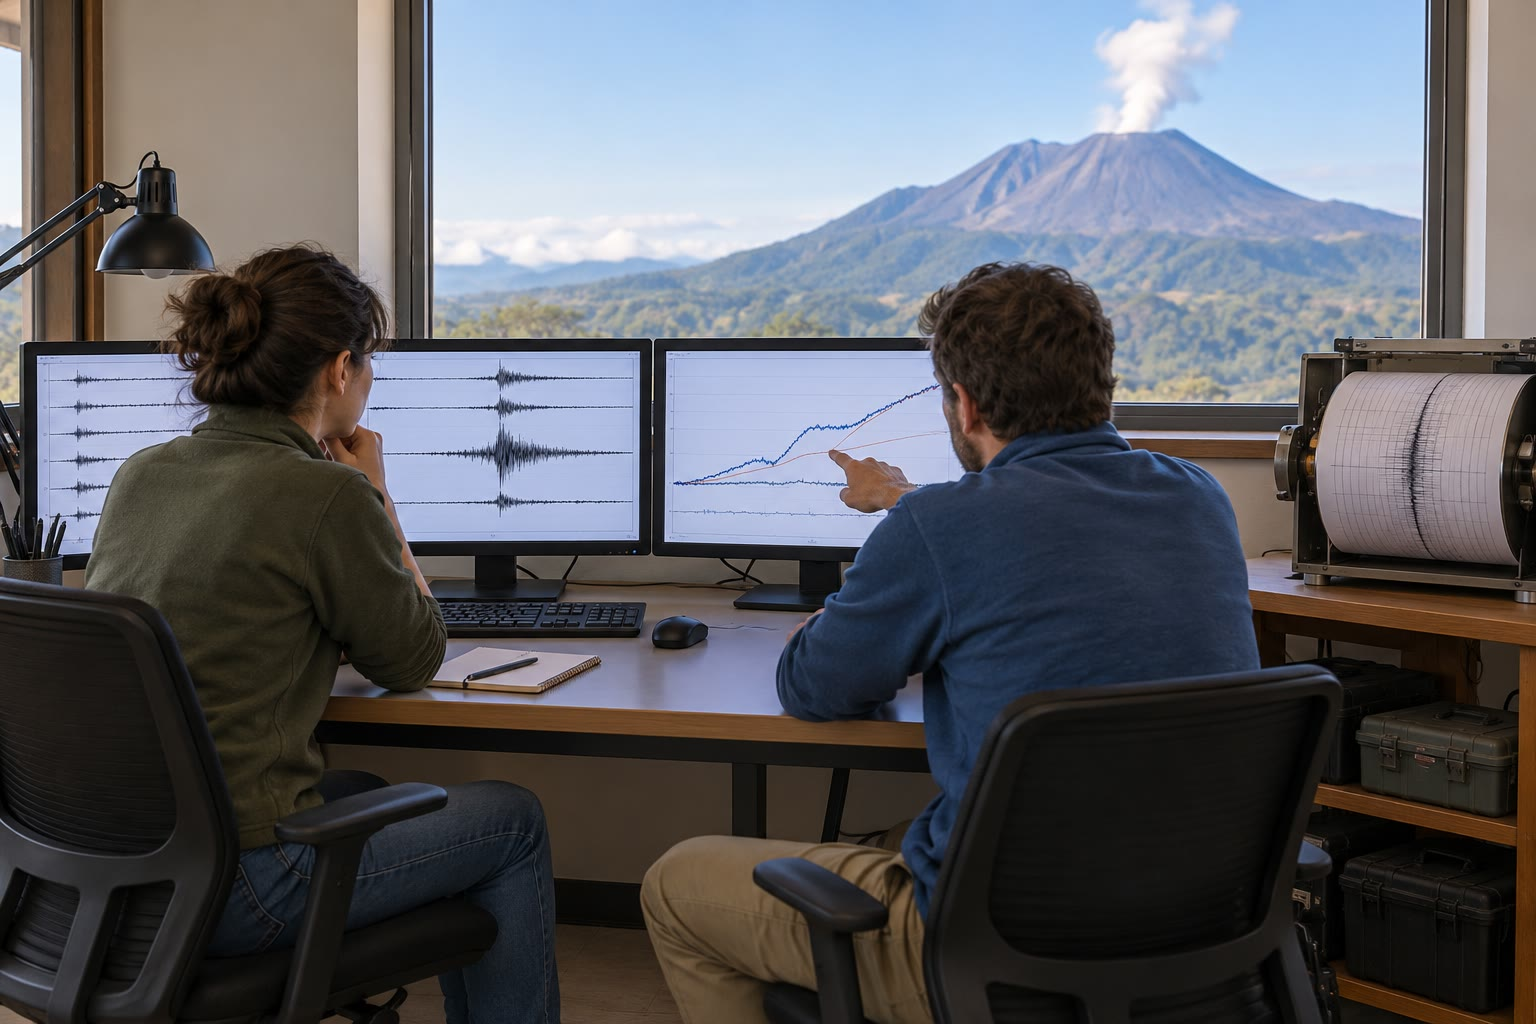
\includegraphics[width=\linewidth]{images/book4/ai/b2-volcano-observatory.jpg}
\par\smallskip{\scriptsize Para ilmuwan meninjau rekaman seismik di sebuah observatorium
gunung api (ilustrasi buatan AI).}
\end{minipage}
\end{inthefield}
% ledger: hvo:alert-levels

\section{Latihan}

\begin{exercise}[$\star$]\label{exo:b2:eruptive-styles:1}
Berikan VEI yang ditunjukkan oleh volume total \omterm{def:b2:eruptive-styles:tephra}{tefra} saja untuk: (a) abu
Gunung St.~Helens, 18 Mei 1980, \qty{1.3}{km^3}; (b) jatuhan Lapisan~5 Cotopaxi,
\qty{0.29}{km^3}; (c) erupsi kecil sebesar \qty{2e6}{m^3}. (d) Material
yang dilontarkan Pinatubo pada tahun 1991 dinyatakan ``lebih dari \qty{5}{km^3}'', tetapi
erupsi itu bernilai VEI~6. Volume total berapa yang sedikitnya tersirat dari nilai itu?
\end{exercise}
% ledger: usgs:vei-criteria, usgs:msh-1980-ash, biass19:layer5, usgs:pinatubo-1991

\begin{exercise}[$\star$]\label{exo:b2:eruptive-styles:2}
Namailah setiap \omterm{def:b2:eruptive-styles:tephra}{piroklas}: (a) serpih kaca sepanjang \qty{0.5}{mm}; (b) fragmen batu apung
selebar \qty{3}{cm}; (c) kepingan bersudut lava tua selebar \qty{20}{cm};
(d) gumpalan berbentuk gelendong sepanjang \qty{8}{cm} dengan ujung-ujung terpilin.
\end{exercise}
% ledger: nps:pyroclast-sizes

\begin{exercise}[$\star$]\label{exo:b2:eruptive-styles:3}
Dengan $H = 0.304\,Q^{0.241}$ ($H$ dalam kilometer di atas lubang kepundan, $Q$ dalam
\unit{kg/s}): (a) hitunglah $H$ untuk $Q = \qty{e6}{kg/s}$ dan \qty{e8}{kg/s};
(b) hitunglah laju erupsi massa yang tersirat dari kolom setinggi \qty{35}{km}, dan
intensitasnya $I = \log_{10}Q + 3$; (c) dengan faktor berapa $Q$ berubah jika tinggi yang terukur
\qty{20}{\percent} terlalu tinggi?
\end{exercise}
% ledger: aubry23:fits, brown14:record

\begin{exercise}[$\star$]\label{exo:b2:eruptive-styles:4}
Jatuhan Lapisan~5 Cotopaxi memiliki volume total \qty{0.29}{km^3}. Dengan mengambil
massa jenis total \qty{1000}{kg/m^3} untuk endapan dan \qty{2500}{kg/m^3} untuk
\omterm{def:b2:magma-emplacement:magma}{magma}, hitunglah volume ekuivalen batuan padatnya, massanya, dan magnitudonya
$M = \log_{10}m - 7$.
\end{exercise}
% ledger: biass19:layer5, brown14:record

\begin{exercise}[$\star\star$]\label{exo:b2:eruptive-styles:5}
Sebuah endapan jatuhan setebal \qty{40}{cm} pada isopak $\sqrt A = \qty{5}{km}$
dan \qty{10}{cm} pada isopak $\sqrt A = \qty{15}{km}$, dan menipis sebagai satu
eksponensial. Hitunglah $k$, $T_0$, jarak paruh ketebalan $\ln 2/k$, volume
total, dan VEI-nya.
\end{exercise}

\begin{exercise}[$\star\star$]\label{exo:b2:eruptive-styles:6}
(a) Tunjukkan bahwa volume di dalam isopak $x = \sqrt A$ sebuah endapan yang menipis
sebagai $T_0e^{-kx}$ adalah $\frac{2T_0}{k^2}[1 - (1 + kx)e^{-kx}]$. (b) Selesaikan $(1 + u)e^{-u} =
1/2$ hingga tiga angka penting dengan substitusi berulang atau bagi dua. (c) Untuk
endapan pada \cref{exo:b2:eruptive-styles:5}, di luar isopak mana separuh volumenya terletak? Bandingkan
dengan jarak isopak terluar yang dipetakan dari lubang kepundan.
\end{exercise}

\begin{exercise}[$\star\star$]\label{exo:b2:eruptive-styles:7}
Sebuah \omterm{def:b2:magma-emplacement:magma}{magma} riolit pada \qty{850}{\celsius} (\qty{1123}{K}) mengandung
\qty{5.0}{\percent} air, dengan kelarutan $s = 0.444$ persen per
$\sqrt{\unit{MPa}}$; lelehannya bermassa jenis \qty{2300}{kg/m^3}. (a) Hitunglah
tekanan jenuhnya, dan kedalaman tempat tekanan itu tercapai untuk gradien
tekanan \qty{0.025}{MPa/m}. (b) Hitunglah fraksi volume gas pada
\qty{10}{MPa} jika gas tetap berada dalam \omterm{def:b2:magma-emplacement:magma}{magma} ($R = \qty{8.314}{J/(mol.K)}$, $M =
\qty{0.018015}{kg/mol}$). (c) Mengapa \omterm{def:b2:magma-emplacement:magma}{magma} basal jauh lebih jarang terfragmentasi,
padahal pada \qty{1}{MPa} basal sistem tertutup dengan \qty{1}{\percent}
air akan berupa \qty{92}{\percent} gas?
\end{exercise}
% ledger: moore98:h2o, cassidy18:fragmentation, cassidy18:ascent

\begin{exercise}[$\star\star$]\label{exo:b2:eruptive-styles:8}
(a) Sebuah \omterm{prop:b2:eruptive-styles:mogi}{sumber Mogi} pada kedalaman \qty{5}{km} bertambah \qty{e7}{m^3}. Hitunglah
pengangkatan di atasnya ($\nu = 0.25$). (b) Gembungan lain turun menjadi separuh maksimumnya
\qty{3.8}{km} dari pusatnya: berapa kedalaman sumbernya? (c) Berapa fraksi
pengangkatan maksimum yang terlihat oleh sebuah stasiun pada jarak mendatar sama dengan kedalaman
sumber?
\end{exercise}
% ledger: dmodels:mogi

\begin{exercise}[$\star\star$]\label{exo:b2:eruptive-styles:9}
Sebuah ledakan Vulkano melontarkan blok-blok keluar dari kawah. Dengan mengabaikan hambatan udara
dan tinggi bibir kawah, hitunglah jangkauan terbesar blok yang dilontarkan
dengan \qty{100}{m/s}, lalu dengan \qty{200}{m/s} ($g = \qty{9.81}{m/s^2}$). Apakah hambatan
udara membuat jangkauan ini menjadi batas atas atau batas bawah? Mengapa zona bahaya
balistik di sekitar lubang kepundan sebanding dengan kuadrat kecepatan lontar?
\end{exercise}

\begin{exercise}[$\star\star\star$]\label{exo:b2:eruptive-styles:10}
(a) Turunkan volume endapan dengan dua segmen eksponensial yang diberikan dalam
kotak metode, dengan menganggap ketebalannya kontinu di tempat kedua garis berpotongan. (b) Untuk
jatuhan Lapisan~5 Cotopaxi, segmen-segmen yang dicocokkan adalah $T = \qty{1285}{cm}\times
e^{-0.365x}$ dan segmen distal dengan kemiringan $k_2 = \qty{0.138}{km^{-1}}$, yang berpotongan pada
$X = \qty{8.56}{km}$. Hitunglah volumenya, dan bagian volume di luar titik
potong itu.
\end{exercise}
% ledger: biass19:layer5

\begin{exercise}[$\star\star\star$]\label{exo:b2:eruptive-styles:11}
(a) Dengan \cref{prop:b2:eruptive-styles:plume}, dengan faktor berapa tinggi
kolom naik jika laju erupsi dikalikan 100? Bandingkan dengan
eksponen empiris $0.241$ dan $0.226$. (b) Ke arah mana atmosfer yang terstratifikasi
lebih kuat mengubah tinggi itu, dan seberapa besar jika $N$ bertambah
\qty{20}{\percent}? (c) Berikan dua alasan mengapa eksponen yang terukur dapat lebih kecil daripada
$1/4$.
\end{exercise}
% ledger: aubry23:fits

\begin{exercise}[$\star\star\star$]\label{exo:b2:eruptive-styles:12}
Katalog global mencantumkan 132 erupsi VEI~4 atau lebih yang dimulai antara 1500
dan 1899, dan 95 antara 1900 dan 2024. (a) Hitunglah laju per abad pada setiap
periode. (b) Jika laju sejak 1900 adalah laju yang sebenarnya, berapa fraksi erupsi
terdahulu yang tercatat? (c) Sebuah studi erupsi besar menemukan 21 erupsi berkekuatan
magnitudo 4 hingga 4.9 per abad antara 1500 dan 1900 dan 56 sejak 1900; bandingkan.
(d) Mengapa fraksi ini bergantung pada ukuran erupsi?
\end{exercise}
% ledger: data:b4-gvp-eruptions, brown14:record

\section{Soal: Membaca endapan Plini}

\begin{problem}[{Soal akhir pekan --- dari isopak jatuhan batu apung hingga besarnya
erupsi, tinggi kolomnya, dan seberapa sering erupsi semacam itu
terjadi}]
\label{pb:b2:eruptive-styles:1}
Sebuah gunung api khayalan telah meninggalkan jatuhan batu apung dari satu fase Plini yang
berlangsung \qty{10}{\hour}. Isopaknya, setelah pemanjangan oleh angin dihilangkan dengan
memakai akar kuadrat luasnya, adalah:
\begin{center}
\small
\begin{tabular}{lccccc}
\hline
$\sqrt A$ (\unit{km}) & 10 & 20 & 40 & 80 & 120 \\
ketebalan $T$ (\unit{cm}) & 200 & 100 & 48 & 14 & 4.0 \\
\hline
\end{tabular}
\end{center}
Data: massa jenis total endapan \qty{900}{kg/m^3}; massa jenis \omterm{def:b2:magma-emplacement:magma}{magma}
\qty{2400}{kg/m^3}; tinggi kolom yang diukur dari klas terbesar,
\qty{31}{km} di atas lubang kepundan; tropopause pada \qty{16}{km}. Gunakan $H =
0.304\,Q^{0.241}$ dan $H = 0.345\,Q^{0.226}$ ($H$ dalam kilometer, $Q$ dalam
\unit{kg/s}).

\medskip\noindent\textbf{Bagian I --- Endapannya.}
\begin{enumerate}
\item Hitunglah $\ln T$ untuk setiap isopak dan tunjukkan bahwa titik-titiknya terletak pada dua
segmen lurus jika diplot terhadap $\sqrt A$. Di mana patahannya?
\item Hitunglah kemiringan $k_1$ dan titik potong $T_0$ segmen proksimal
yang melalui dua isopak pertama.
\item Garis kuadrat terkecil melalui ketiga isopak distal adalah $T =
\qty{167}{cm}\times e^{-0.0311\sqrt A}$. Periksalah bahwa garis itu lewat dalam selisih
\qty{5}{\percent} dari setiap isopak itu.
\item Hitunglah nilai $\sqrt A$ tempat kedua garis berpotongan.
\item Hitunglah jarak paruh ketebalan $\ln 2/k$ kedua segmen.
\item Hitunglah volume yang akan dimiliki endapan itu jika endapan menipis dengan kemiringan
proksimal di mana-mana.
\item Hitunglah volume total dengan kedua segmen, dan bagian yang disumbangkan oleh
koreksi untuk segmen distal yang lebih landai.
\item Dengan faktor berapa volume itu akan ditaksir terlalu rendah jika hanya endapan
proksimal yang dipetakan? Mengapa hal itu merupakan risiko nyata bagi endapan tua?
\end{enumerate}

\noindent\textbf{Bagian II --- Besarnya erupsi.}
\begin{enumerate}[resume]
\item Berikan VEI erupsi itu.
\item Hitunglah volume ekuivalen batuan padat.
\item Hitunglah massa yang dierupsikan.
\item Hitunglah magnitudo $M = \log_{10}m - 7$.
\item Berapa kali lebih besar endapan ini daripada jatuhan abu Gunung St.~Helens tahun 1980,
\qty{1.3}{km^3}?
\item Tinggi kolom berapa yang dikaitkan tabel VEI dengan erupsi ini, dan
gaya apa?
\end{enumerate}

\noindent\textbf{Bagian III --- Kolomnya.}
\begin{enumerate}[resume]
\item Hitunglah laju erupsi massa rata-rata selama fase Plini, dan
intensitasnya $I = \log_{10}Q + 3$.
\item Hitunglah tinggi kolom yang diramalkan oleh hukum empiris pertama.
\item Hal yang sama dengan hukum kedua.
\item Bandingkan dengan \qty{31}{km} yang diukur dari klas, mengingat sebaran
hukum-hukum itu.
\item Laju erupsi massa berapa yang tersirat dari \qty{31}{km} menurut hukum pertama? Dengan
faktor berapa laju itu berbeda dari laju pada pertanyaan~15, dan apa yang mungkin menjelaskannya?
\item Apakah kolom itu menyuntikkan gas ke stratosfer? Apa yang dapat menyusul bagi
iklim, dan gas apa yang menjadi kuncinya?
\end{enumerate}

\noindent\textbf{Bagian IV --- Seberapa sering?}
\begin{enumerate}[resume]
\item Dari hitungan katalog (399 erupsi VEI $\ge 3$ dari 1950 hingga
2024, 95 erupsi VEI $\ge 4$ dari 1900, 22 erupsi VEI $\ge 5$ dari 1800, 8 erupsi VEI $\ge 6$ dari
1500, semua jendela berakhir pada 2024 termasuk), hitunglah keempat laju tahunan dan
logaritmanya.
\item Periksalah bahwa garis $\log_{10}\lambda_v = 3.28 - 0.85\,v$ lewat dalam selisih
\qty{10}{\percent} dari setiap laju.
\item Mengapa setiap jendela dimulai lebih jauh ke belakang untuk erupsi yang lebih besar?
\item Dari garis itu, hitunglah laju erupsi VEI $\ge 5$, periode ulang
rata-ratanya, dan peluang sedikitnya satu erupsi dalam 10 tahun mendatang.
\item Dari garis itu, hitunglah laju erupsi VEI $\ge 7$ dan bandingkan
dengan dua erupsi yang tercatat sejak tahun 1000.
\item Dari garis itu, hitunglah laju erupsi VEI $\ge 6$ dan
peluang, dalam persen, sedikitnya satu erupsi di suatu tempat di Bumi dalam 100
tahun mendatang, yaitu angka kunci soal ini. Asumsi apa yang menjadi dasarnya?
\end{enumerate}
\end{problem}
